\section {PlanesGraphicsScene}

Similar to the PlanesWidget variant, the main window of the project is an object of a class derived from QMainWindow. In the constructor it creates the View - PlanesGSView - and the controller - PlaneRound - the game engine. 

\begin{figure}[h]
	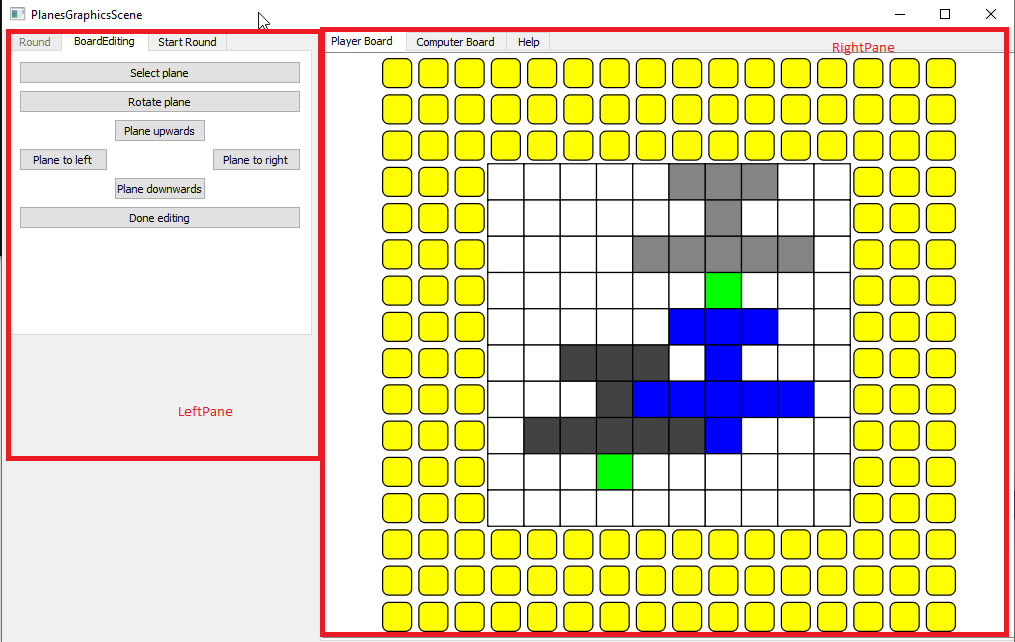
\includegraphics[width = \textwidth]{PlanesGraphicsScene_BoardEditing_WidgetNames.png}
	\caption{Simplified Layout of PlanesGraphicsScene}
	\label{fig:planesgraphicsscene_boardediting_widgetnames}
\end{figure}

The member variables for the PlanesGSView are:

\begin{lstlisting}

	//PlaneGrid objects manage the logic of a set of planes on a grid
	//as well as various operations: save, remove, search, etc.
	PlaneGrid* m_playerGrid;
	PlaneGrid* m_computerGrid;
	
	//PlaneRound is the object that coordinates the game
	PlaneRound* m_round;
	
	LeftPane* m_LeftPane;
	RightPane* m_RightPane;

\end{lstlisting}

Better as in the PlanesWidget project, the ComputerLogic object is not extracted from the PlaneRound anymore, only the two PlaneGrid objects are, which is still not satisfactory. The widgets composing the GUI are grouped under two principal widgets: LeftPane and RightPane.

The layout of the PlanesGSView is defined as follows:

\begin{lstlisting}
	CustomHorizLayout* hLayout = new CustomHorizLayout(this);
	m_LeftPane = new LeftPane(this);
	m_LeftPane->setMinWidth();
	//m_LeftPane->setSizePolicy(QSizePolicy::Fixed, QSizePolicy::Expanding);
	
	m_RightPane = new RightPane(*m_playerGrid, *m_computerGrid, this);
	m_RightPane->setMinWidth();
	
	hLayout->addWidget(m_LeftPane);
	hLayout->addWidget(m_RightPane);
	setLayout(hLayout);
\end{lstlisting} 

In principle it is a customized horizontal layout containing the LeftPane and RightPane widgets (see Figure \ref{fig:planesgraphicsscene_boardediting_widgetnames}). 


\subsection{Qt Concepts}

\subsubsection{Implementing a Custom Layout}

